\chapter{DATA C100: Estimators, Bias, and Variance}

We have now find many ways to compute and summarize random variable via statistical and mathematical means, as outlined in A Survey on Random Variables and to be performed in future chapters. \\
However, data science per se often concern with another issue: sampling. While we may obtain the distribution of some random sample we acquire, we do not necessarily then recognize the distribution of a population. \\
So the essential question this chapter's contents revolve around would then be:
\begin{center}
    ``Can we infer or estimate the properties of a population based on the distribution of our samples?''
\end{center}

\section{Sample Statistics}
Consider that each datapoints in our sample is some IID random variable drawn from the population distribution. \\
Then, we may consider the statistics of this sample to be a random variable as well, as the possible samples themselves are driven from random experiments and will serve as the domain of these random-variable styled statistics.

Here, an incredibly practical theorem would then answer the question we threw at the beginning of the chapter.
\begin{ln-theorem}{Central Limit Theorem}{}
    Regardless of the population that samples are drawn from, if an IID sample of size $n$ is large, the probability distribution of the sample mean is roughly normal with mean $\mu$, standard devaition $\frac{\sigma}{\sqrt{n}}$. \\
    Here, $\mu$ is the population mean, and $\sigma$ is population standard deviation.
\end{ln-theorem}
A much formal introduction to Central Limit Theorem will be performed in the last few chapters for COMPSCI 70.

We may then, along the help of Central Limit Theorem, define the ``average sample'' that a population possibly acquires:
\begin{ln-define}{Sample Mean}{}
    Consider an IID sample $X_1, \dots, X_n$ drawn from numerical population with mean $\mu$, standard deviation $\sigma$, then the sample mean is a sample defined mathematically as:
    \[
        \overline{X_n} = \frac{1}{n} \sum_{i = 1}^n X_i
    \]
    Where we may then compute the expectation and variances of this sample mean to be:
    \begin{align*}
        \E[\overline{X_n}] &= \frac{1}{n} \sum_{i = 1}^n \E[X_i] \\
        &= \frac{1}{n} (n \mu) = \mu
    \end{align*}
    Meanwhile,
    \begin{align*}
        Var(\overline{X_n}) &= \frac{1}{n^2} \sum_{i = 1}^n Var(X_i) \\
        &= \frac{1}{n^2} n \sigma^2 = \frac{\sigma^2}{n} \\
        SD(\overline{X_n}) &= \frac{\sigma}{\sqrt{n}}
    \end{align*}
\end{ln-define}
The performance of Central Limit Theorem in realistic constraints is very dependent on the ambiguity in its description, ``a large $n$''. \\
What is the demand on the size of $n$ for CLT to work properly by description and present us some convenient normal distribution? \\
This would, in fact, depend on the skewness of population. If the population is roughly symmetric and unimodal, for example, the required value of $n$ becomes remarkably small. Otherwise, a large $n$ would still be required.

The use of sample mean as a statistic is to serve as an estimation of population mean: we consider the collaborative mean and variance of multiple samples to be a good estimate for that of the population. \\
But before discussinf the sample mean as an estimation, we should first switch gears and explore the concept of ``estimation'' in the context of modeling: that is, the work of inference.

\section{Prediction and Inference in Modeling}
A model is constructed for two dominant reasons:
\begin{bindenum}
    \item \textbf{Prediction}: The model offers a prediction for the response of an unseen data entry.
    \item \textbf{Inference}: Extracting conclusions about the underlying relationship between predictor features and responses from a model's inner settings and parametric properties.
\end{bindenum}
Then, in the context of modeling, the work of estimation as addressed in prior section to infer about population parameters given some random sample. This is otherwise called ``statistical inference''.

\subsection{Estimator and Bias-Variance Tradeoff}
The performance of an estimator variable can be assessed at the following perspectives:
\begin{bindenum}
    \item \textbf{Bias}: Does the estimator variable offer the right answer (value of estimated parameter) on average?
    \item \textbf{Variance}: What is the variability of the estimator's answer?
    \item \textbf{Risk}: How close is the work of estimator to the parameter it estimates?
\end{bindenum}
All of which offer some mathematical quantification to evaluate the estimator's performance.
\begin{ln-define}{Bias of Estimator}{}
    The bias of an estimator measures its average deviation from the true value (parameter):
    \[
        Bias(\hat{\theta}) = \E[\hat{\theta} - \theta] = \E[\hat{\theta}] - \theta
    \]
    Because the sample mean's average is $\E[\hat{\theta}] = \mu$, directly equivalent to the population mean, the sample mean served as an unbiased estimator.
\end{ln-define}
\begin{ln-define}{Risk of Estimator}{}
    The risk of the estimator can be expressed via some loss function like MSE as:
    \[
        MSE(\hat{\theta}) = \E[{(\theta - \hat{\theta})}^2]
    \]
    And if the estimator $\hat{\theta}$ is unbiased, we may learn that $\E[\hat{\theta}] = \theta$, making the risk of an estimator its variance.
\end{ln-define}
In the case that the estimator is not unbiased, we can then decompose MSE risk of the estimator as follows:
\begin{align*}
    b &= \E[\hat{\theta}] - \theta \\
    MSE(\hat{\theta}) &= \E[{(\hat{\theta} - \theta)}^2] \\
    &= \E[{(\hat{\theta} - \E[\hat{\theta}] + b)}^2] \\
    &= \E[{(\hat{\theta} - \E[\hat{\theta}])}^2] + b^2 + 2b\E[(\hat{\theta} - \E[\hat{\theta}])] \\
    &= b^2 + Var(\hat{\theta})
\end{align*}
We call this result the \textbf{Bias-Variance Decomposition}.

\subsection{Estimation Error for Modeling}
Let us apply the notion of ``estimation'' onto choosing model relationships. \\
Say, that the response variable $Y$ is to predicted by some expression:
\[Y = g(x) + \epsilon\]
for some $g$ that estiamtes the true relationship between $x$ and $Y$. Then, $\epsilon$ would represent some random error or noise that are expectedly zero-mean and IID across individual datapoints.
From there, some model for predictions based on observed samples are created: $\hat{Y}(x)$, which once again estimates the true relationship that $g$ is. Evidently, at every set of predictor features $x$, our prediction for the response would then be $\hat{Y}(x)$. \\
Naturally, these estimative models will then also have their own set of optimal parameters to minimize some loss; this fact we will mathematically express here for:
\[\hat{Y}(x) = f_{\hat{\theta}}(x)\]

\section{Bias-Variance Tradeoff}
Let us combine the prior subsections' work to discuss the essential phenomenon and guideline of model training: bias-variance tradeoff, which outlines the tradeoff of model characteristics that determine the overfitting inclinations of models.

From prior work, we can discover the bias-variance decomposition of some \textbf{model risk} (the risk of a model). \\
Model risks are composed of:
\begin{bindenum}
    \item \textbf{Observation Variance}, noted by the random noise $\epsilon$ found from observation; once again, expectedly zero-mean.
    \item \textbf{Model Variance}, the variance that model presents with the random samples it can utilize.
    \item \textbf{Model Bias}, as our model will have some deviation with the true estimated relationship $g$.
\end{bindenum}
And by prior work we have understood that:
\[
    \text{model risk} = \text{observation variance} + {(\text{model bias})}^2 + \text{model variance}
\]
Let us then discuss these aspects of model risk:
\begin{ln-define}{Observation Variance}{}
    Observation Variance is the variance of random error, mathematically denoted as:
    \[\sigma^2\]
    which originates from measurement error and noise-behaving missing information. \\
    While observation variance can be reduced via more precise measurements, this is often beyond the control of scientists.
\end{ln-define}
\begin{ln-define}{Model Variance}{}
    Since our fitted model $\hat{Y}$ is on a random sample, the deviations of possible random samples to fit model on would present different models. \\
    This varaince of our prediction at a fixed $x$ is known as model variance, mathematically denoted as:
    \[Var(\hat{Y(x)})\]
    Model variance can originate from overfitting, where small differences in random samples lead to huge deviations in some fitted model due to the models being overfitted to their respective random training samples. \\
    To reduce model variance, one may reduce model complexity (as a method to inhibit overfitting), as well as preventing the model to fit the observation variance and noises.
\end{ln-define}
\begin{ln-define}{Model Bias}{}
    The model bias is the difference between our predicted response and the true value of response, mathematically defined as:
    \[\text{model bias} = \E[\hat{Y(x)}] - g(x)\]
    Here, bias is an average measure for some fixed $x$, just as model variance is presented. \\
    By the nature of bias being ``estimation minus real'', a positive bias expresses overestimation, while negative bias expresses underestimation. The opposite logic was applied on residuals. \\
    Overall, model bias can originate from underfitting, as well as from the lack of domain knowledge that a model requires to operate well. To reduce model bias, one can increase the model complexity and involve domain knowledge to construct better prioris for prediction work.
\end{ln-define}
Therefore, summarizing the above, we see that the bias-variance decomposition for some model risk can be summarized mathematically as:
\[
    \E[{(Y - \hat{Y}(x))}^2] = \sigma^2 + {(\E[\hat{Y}(x)] - g(x))}^2 + Var(\hat{Y}(x))
\]
as paralleling the prior statement:
\[
    \text{model risk} = \text{observation variance} + {(\text{model bias})}^2 + \text{model variance}
\]
Therefore, we obtain some important conclusions:
\begin{bindenum}
    \item As models increase in complexity, they overfit and present higher model variance.
    \item As models decrease in complexity, they underfit and present higher model bias.
    \item Observation variance is fundamentally irereducible.
    \item Model risk is a fixed constant due to it being some expectation of random variable.
\end{bindenum}
Consequentially: when tuning a model, \textbf{either its bias or its variance increase}.

This leads to the famous diagram and saying of \textbf{Bias-Variance Tradeoff}:
\begin{ln-fig}{Bias-Variance Tradeoff, DATA C100}{}
    \begin{center}
        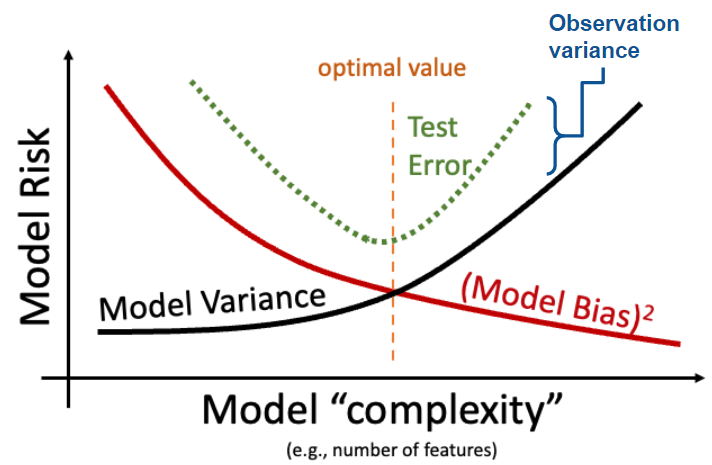
\includegraphics[scale=0.8]{figs/ln09/bv-tradeoff.png}
    \end{center}
\end{ln-fig}
